\documentclass{mc2015}

%%%%%%%%%%%%%%%%%%%%%%%%%%%%%%%%%%%%%%%%%%%%%%%%%%%%%%%%%%%%%%%%%%%%%
\usepackage[T1]{fontenc}         % Use T1 encoding instead of OT1
\usepackage[utf8]{inputenc}      % Use UTF8 input encoding
\usepackage{microtype}           % Improve typography
\usepackage{booktabs}            % Publication quality tables
\usepackage{amsmath}
\usepackage{graphicx}
\usepackage{float}
\usepackage[exponent-product=\cdot]{siunitx}
\usepackage[colorlinks,breaklinks]{hyperref}
\hypersetup{linkcolor=black, citecolor=black, urlcolor=black}

\usepackage{lipsum}

\def\equationautorefname{Eq.}
\def\figureautorefname{Fig.}

%%%%%%%%%%%%%%%%%%%%%%%%%%%%%%%%%%%%%%%%%%%%%%%%%%%%%%%%%%%%%%%%%%%%%
% Insert authors' names and short version of title in lines below

\authorHead{Chris Dances, Vince Mousseau, Maria Avramova}
\shortTitle{Transient Verification of COBRA-TF}

%%%%%%%%%%%%%%%%%%%%%%%%%%%%%%%%%%%%%%%%%%%%%%%%%%%%%%%%%%%%%%%%%%%%%
\begin{document}

\title{Initial 1-D Single Phase Liquid Transient Verification of COBRA-TF}

\author{Chris Dances}
\author{Dr. Maria Avramova}
\affil{ Department of Mechanical and Nuclear Engineering \\
  The Pennsylvania State University \\
  137 Reber Building, University Park, PA, 16802, USA \\
  cad39@psu.edu; mna109@psu.edu}

\author{Dr. Vince Mousseau}
\affil{ Computer Science Research Institute \\
  Sandia National Laboratories \\
  1450 Innovation Parkway, Albuquerque, NM 87123, USA \\
  vamouss@sandia.gov
}

\maketitle

\begin{abstract}
Abstract \ldots

\emph{Key Words}: List no more than five key words
\end{abstract}

\clearpage
%%%%%%%%%%%%%%%%%%%%%%%%%%%%%%%%%%%%%%%%%%%%%%%%%%%%%%%%%%%%%%%%%%%%%

%\tableofcontents
%\clearpage
%
%\listoffigures
%\clearpage

%%%%%%%%%%%%%%%%%%%%%%%%%%%%%%%%%%%%%%%%%%%%%%%%%%%%%%%%%%%%%%%%%%%%%
\section{Introduction}

For the past several decades, the primary focus in nuclear engineering within
the United States has been focused on light water reactors (LWR). Commercially,
all nuclear reactors are either boiling water reactors (BWR) or pressurized
water reactors (PWR). Correct computation of the thermal hydraulics within the
reactor core leads to effi- cient design and accuracy in the safety analysis. A
popular subchannel code for modelling the hydrodynamics with in the reactor core
is COBRA-TF. This FORTRAN based code solves 8 conservation equations for liquid,
entrained droplet, and vapor phases in 3-D dimmensions \cite{CTF_Theory}. The
conservation equations analytically reduce into a pressure matrix in a 
semi-implicit  method with rod temperatures solved for explicitly. Because the 
physics are integrated into the numerical solution, the equations  must be
linear and the solution method semi-implicit. With a residual formulation,
greater flexibility and control over the numerical solution is possible.
COBRA-TF was originally written in FORTRAN 77, but over the years has been
partially updated to newer versions of Fortran.

\section{COBRA-TF}

The finite volume structure in COBRA-TF in figure \ref{fig:CTF-Cells} is for a
one-dimmensional channel in the axial direction with n number of cells. The
first and last cells at 0 and n + 1 are ghost cells and act as the boundary
conditions for the problem. Pressure, enthalpy, and density are averaged over
the cell volume and are located at the center of the cell. Mass flow rate and
velocity are located at the faces in between cells. The cells  are represented
with an index i, and the faces with indexes of $i + \frac{1}{2}$ or 
$i-\frac{1}{2}$. This project will initially focus on this 1-D configuration.
Usually the code  is 3-D,  with channels connecting to each other in two more 
dimmensions.

\begin{figure}[!h]
	\centering
	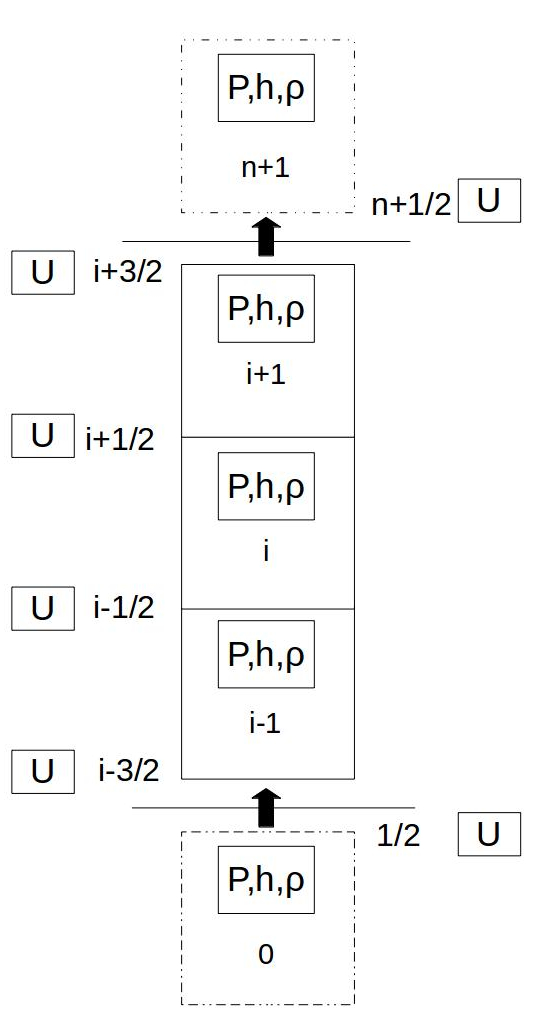
\includegraphics[width=0.30\textwidth]{images/CTF-Cells}
	\caption{The finite volume structure for COBRA-TF}
	\label{fig:CTF-Cells}
\end{figure}

\subsection{1-D Single Phase Liquid Conservation Equations}

The thermal hydraulics of a LWR core is an important part of nuclear
reactor desigin. COBRA-TF solves 8 conservation equations for liquid,
entrained droplet, and vapor phases of water boiling within the rod structure
of a LWR reactor core \cite{CTF_Theory}. Currently, the conservation
equations analytically reduce into a pressure matrix in a semi-implicit
method with rod temperatures solved for explicitly. This work involves
representing the 1-D single phase liquid conservation equations and calculated 
variables in a residual formulation. The full jacobian matrix can then be
built numerically, and  can then either be reduced to a pressure matrix or
solved directly.

The single phase Euler partial differential equations for mass
\eqref{eq:pde_mass}, momentum \eqref{eq:pde_momentum}, and energy
\eqref{eq:pde_energy} corresond to the unknown variables density $\rho$,
velocity $u$, pressure $P$, and enthalpy $h$. The first terms in each of the
equations are temporal terms. The rest of the terms are steady state spatial
terms. 
    
    \begin{equation}
    	\label{eq:pde_mass}
    	\frac{ \partial \rho}{\partial t} + \bigtriangledown \rho u = 0
    \end{equation}
    
    \begin{equation}
    	\label{eq:pde_momentum}
    	\frac{ \partial \rho u}{\partial t} + \bigtriangledown \rho u^{2} +
    	\bigtriangledown P - \rho g  = 0
    \end{equation}
    
    \begin{equation}
    	\label{eq:pde_energy}
    	\frac{ \partial \rho h}{\partial t} -
    	\frac{ \partial  P}{\partial t} + 
    	\bigtriangledown ( \rho  u h )
    	= 0
    \end{equation}
    
\subsection{Modified Equation Analysis}
    
    For this isokinetic problem, the original mass balance equation can be re-written to 
    look like equation \ref{CAD:eq:isokinetic_start}. Using upwinding, the finite difference
    can be written to look like equation \ref{CAD:eq:mass_isok_fd}. A second order Taylor 
    series approximation can be used for $\rho_{i}^{n+1}$ and $\rho_{i-1}^{n}$ as shown 
    in equations \ref{CAD:eq:rho_taylor_series_time} and \ref{CAD:eq:rho_taylor_series_space} 
    respectively. The higher order terms ($O(\Delta x^{2},\Delta t^{2} )$) are
    not taken into account for this approximation. The Taylor series
    approximations can then be substituted into \ref{CAD:eq:mass_isok_fd} to yield
    \ref{CAD:eq:MEA_start}. This is the beginning of the modified equation analysis.
    The goal will be to isolate the original PDE and define the truncation error.
    
    \begin{equation}
    	\label{CAD:eq:isokinetic_start}
    	\frac{\partial \rho}{\partial t} + U_{0} \frac{\partial \rho}{\partial x} = 0
    \end{equation}
    
    \begin{equation}
    	\label{CAD:eq:mass_isok_fd}
    	\frac{ \rho_{i}^{n+1} - \rho_{i}^{n} }{\Delta t} 
    	+ U_{0} \frac{\rho_{i}^{n} - \rho_{i-1}^{n}}{\Delta x} = 0
    \end{equation}
    
    \begin{equation}
    	\label{CAD:eq:rho_taylor_series_time}
    	\rho_{i}^{n+1} =  \rho_{i}^{n} + 
    	\frac{\partial \rho}{\partial t} \Delta t +
    	\frac{1}{2} \frac{\partial^2 \rho}{\partial t^2} \Delta t^2 + O(\Delta t^{3})
    \end{equation}
    
    \begin{equation}
    	\label{CAD:eq:rho_taylor_series_space}
    	\rho_{i-1}^{n} =  \rho_{i}^{n} - 
    	\frac{\partial \rho}{\partial x} \Delta x +
    	\frac{1}{2} \frac{\partial^2 \rho}{\partial x^2} \Delta x^2 + O(\Delta x^{3})
    \end{equation}
    
    The lengthy equation \ref{CAD:eq:MEA_start} can be reduced to equation
    \ref{CAD:eq:MEA_p0} since the $\rho_{i}^{n}$ terms subtract out and the $\Delta
    t$ and $\Delta x$ terms in the denominator cancel out. This reduced equation
    can the be re-written into equation \ref{CAD:eq:MEA_p1}, with the original PDE
    followed by the truncation terms. Notice how the terms on the right are
    dependent on both the numerical spacing $\Delta t$ and $\Delta x$, but also
    on the second derivatives of density with respect to space and time.
    
    \begin{equation}
    	\label{CAD:eq:MEA_start}
    	\frac{ \left( \rho_{i}^{n} + \frac{\partial \rho}{\partial t} \Delta t +
    	\frac{1}{2} \frac{\partial^2 \rho}{\partial t^2} \Delta t^2 \right)-\rho_{i}^{n} }{\Delta t} 
    	+ U_{0} \frac{\rho_{i}^{n} - \left( \rho_{i}^{n} -  \frac{\partial \rho}{\partial x} \Delta x + 
    	\frac{1}{2} \frac{\partial^2 \rho}{\partial x^2} \Delta x^2 \right)}{\Delta x} 
    	+ O(\Delta x^{2},\Delta t^{2}) 
    	= 0
    \end{equation}
    
    \begin{equation}
    	\label{CAD:eq:MEA_p0}
    	 \frac{\partial \rho}{\partial t}  + \frac{1}{2} \frac{\partial^2 \rho}{\partial t^2} \Delta t +
    	 U_{0} \left(   \frac{\partial \rho}{\partial x}  - \frac{1}{2} \frac{\partial^2 \rho}{\partial x^2} \Delta x \right) 
    	 + O(\Delta x^{2},\Delta t^{2}) 
    	 = 0
    \end{equation}
    
    \begin{equation}
    	\label{CAD:eq:MEA_p1}
    	 \frac{\partial \rho}{\partial t}  +  U_{0} \frac{\partial \rho}{\partial x} + 
    	 \frac{1}{2} \frac{\partial^2 \rho}{\partial t^2} \Delta t -
    	   U_{0}  \frac{1}{2} \frac{\partial^2 \rho}{\partial x^2} \Delta x  
    	   + O(\Delta x^{2},\Delta t^{2}) = 0 
    \end{equation} \linebreak
    
    Before we can procede, we need to take the derivative of the original PDE with respect
    to space and time as shown in equations \ref{CAD:eq:mass_dt} and  \ref{CAD:eq:mass_dx} 
    respectively. These two derivatives can substitute into each other using the common 
    term $\frac{\partial^2 \rho}{\partial x \partial t}$. The second derivatives of density with 
    respect to space and time are therefore related by the velocity squared as
    shown by equation \ref{CAD:eq:mass_second_derivatives}.
    
    \begin{equation}
    \label{CAD:eq:mass_dt}
    	 \frac{\partial^2 \rho}{\partial t^2} + U_{0} \frac{\partial^2 \rho}{\partial x \partial t} = 0
    \end{equation}
    
    \begin{equation}
    \label{CAD:eq:mass_dx}
    	 \frac{\partial^2 \rho}{\partial t \partial x} + U_{0} \frac{\partial^2 \rho}{\partial x^2} = 0
    \end{equation}
    
    \begin{equation}
    \label{CAD:eq:mass_second_derivatives}
    	 \frac{\partial^2 \rho}{\partial t^2} =  U_{0}^2 \frac{\partial^2 \rho}{\partial x^2}
    \end{equation} \linebreak
    
    This relationship can then be substituted back into equation \ref{CAD:eq:MEA_p1}, 
    which can be reduced to equation \ref{CAD:eq:MEA_result} after igonoring the higher
    order terms. The error depends on the CFL number, the axial spacing, and the
    second order derivative of density with respect to space. This derivative is
    what gives the error the characterisitcs of diffusion. When the CFL number is
    less than one, the error term is negative and the diffusion is dampening. When
    the CFL number is greater than one, the error term becomes positive, and the
    accumulation of the error destabilizes the solution. 
    
    \begin{equation}
    	 \frac{\partial \rho}{\partial t}  +  U_{0} \frac{\partial \rho}{\partial x} - 
    	  \frac{1}{2}  \left(  \Delta x U_{0} \frac{\partial^2 \rho}{\partial
    	  x^2} -   U_{0}^2 \frac{\partial^2 \rho}{\partial x^2} \Delta t  \right) 
    	   + O(\Delta x^{2},\Delta t^{2}) = 0
    \end{equation}
    
    \begin{equation}
    \label{CAD:eq:MEA_result}
    	 \frac{\partial \rho}{\partial t}  +  U_{0} \frac{\partial \rho}{\partial x} - 
    	 \frac{\Delta x U_{0}}{2} \frac{\partial^2 \rho}{\partial x^2}  
    	 \left(  1 - CFL  \right) 
    	 + O(\Delta x^{2},\Delta t^{2})  = 0
    \end{equation}
    
    Modified eqauation analysis can be applied to the energy balance equation
    presented in equation \ref{CAD:eq:MEA_energy}. The energy equation is presented in a form where
    the momentum equation was substituted in as zero and then divided through by
    density. The result presented in equation \ref{CAD:eq:MEA_ene_result} is similar in
    form to the result for the mass balance equation \ref{CAD:eq:MEA_result}.
    
    \begin{equation}
    	\label{CAD:eq:MEA_energy}
    	\frac{\partial h}{\partial t} - \frac{1}{\rho} \frac{\partial P}{\partial t} +
    	U_{0} \frac{\partial h}{\partial x} = 0
    \end{equation}
    
    \begin{equation}
    \label{CAD:eq:MEA_ene_result}
    	\frac{\partial h}{\partial t} - \frac{1}{\rho} \frac{\partial P}{\partial t} +
    	U_{0} \frac{\partial h}{\partial x} - 
    	\frac{\Delta x U_{0}}{2} \frac{\partial^2 h}{\partial x^2}
    	\left( 1 - CFL \right)
    	= 0
    \end{equation}

\subsection{Residual Formulation and Jacobian Construction}

	A residual is simply the difference between the value at some future time
    $n+1$ and the value at the current iteration $k$. This can be applied to
    desired variables as shown in equations
    \eqref{CAD:eq:residual_def:P}, \eqref{CAD:eq:residual_def:h},
    \eqref{CAD:eq:residual_def:u}, and \eqref{CAD:eq:residual_def:rho}. Residuals can
    also be applied to the conservation equations by substituting the definition
    of the residual variables into the conservation equations. This will
    effectively change any variables evaluated at $n+1$ to $k$. Each cell will
    have three residual variables and three residual equations. For the entire
    solution, we will then have a residual variable array $\delta X$, and a
    residual function array $F(X)$ which defines a linear system as seen in 
    equation \eqref{CAD:eq:linear_system}.
        
    \begin{equation}
    	\label{CAD:eq:residual_def:P}
    	\delta P_{i} = P^{n+1}_{i} - P^{k}_{i}
    \end{equation}
    
    \begin{equation}
    	\label{CAD:eq:residual_def:h}
    	\delta h_{i} = h^{n+1}_{i} - h^{k}_{i}
    \end{equation}
    
    \begin{equation}
    	\label{CAD:eq:residual_def:u}
    	\delta u_{i+\frac{1}{2}} = u^{n+1}_{i+\frac{1}{2}} - u^{k}_{i+\frac{1}{2}}
    \end{equation}
    
    \begin{equation}
    	\label{CAD:eq:residual_def:rho}
    	\delta \rho_{i} = \rho^{n+1}_{i} - \rho^{k}_{i}
    \end{equation}
    
    \begin{equation}
    	\label{CAD:eq:linear_system}
    	J \delta X = - F(X)
    \end{equation}
    
    The Jacobian matrix is defined in equation \eqref{CAD:eq:jac_def} as the derivative
    of each response of the function $F_{j}$ with respect to each variable $X_{i}$.
    The derivative can be calculated numerically as shown by equation
    \eqref{CAD:eq:jac_numerical} where $\epsilon$ is a small numerical value. For
    COBRA-TF the equations are linear, and this numerical approximation
    of the Jacobian matrix is exact. This should produce the same jacobian
    matrix that COBRA-TF currently generates analytically. 
    
    \begin{equation}
    	\label{CAD:eq:jac_def}
    	J_{i,j}=\frac{ \partial F_{j}(X)}{\partial X_{i}}
    \end{equation}
    
    \begin{equation}
    	\label{CAD:eq:jac_numerical}
    	J_{i,j}  \approx \frac{F_{j}(X_{i}+\epsilon)-F_{j}(X)}{\epsilon}
    \end{equation}
    
	To build the jacobian matrix, an object oriented class was created that
    contains three arrays. An array that points to the residual functions, an
    array that points to the position within a target variable arrray, and an
    array that has the index that the function is to be evaluated at. These
    lists can be appended to in any order, but have to be appended all at the
    same time so that variables and functions must correspond with each other.
    Then to construct the jacobian matrix, the residual function and residual
    variable arrays can each be looped over to numerically build the jacobian
    matrix as seen in figure \ref{CAD:fig:Jacobian_Setup}. 
    
    \begin{figure}[!h]
    	\centering
    	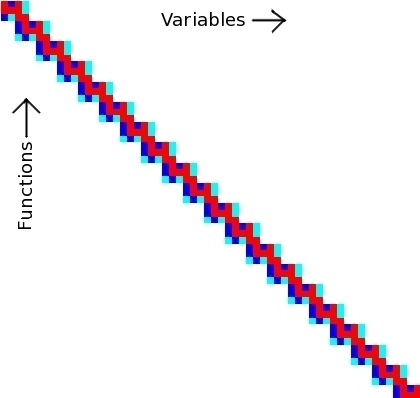
\includegraphics[width=0.45\textwidth]{images/Jacobian_Setup}
    	\caption{Strucutre of the jacobian matrix for single phase liquid}
    	\label{CAD:fig:Jacobian_Setup}
    \end{figure}

\section{Code Verification}

Introduction here \ldots

What is it, what are its objectives \ldots

What distinguishes it from Solution Verification???

\subsection{Software Quality Assurance}

Git, unit tests, code documentation, doxygen, etc.

\subsection{Verification Criteria}

Code verification criteria can be defined to
have the following levels of rigor \cite{Roy:2005:RCS:1082892.1082899}
(cite the original source???)

\begin{itemize}
  \item expert judgement
  \item error quantification
  \item consistencey / convergence
  \item order of accuracy
\end{itemize}

Error quantification, convergence, and order of accuracy will all be used. Order
of accuracy is the most difficult to satisfy and the most sensitive to coding
mistakes.

\subsection{Method of Exact Solutions}

What it is \ldots

How it applies here

Explanations of the expected results \ldots

\section{Solution Verification}

\subsection{Sources of Numerical Error}

Round off error, iterative convergence error.

Discretization error?? (Check with)

\section{Isokinetic Sine Wave Advection Problem}

Needs a figure and a table of parameters. Geometry and reference conditions
should be for a PWR.

The problem is to transiently vary the inlet enthalpy $h$ and inlet mass flow
rate $\dot{m}$ using a smooth trigonometric function so as to keep velocity
constant throughout the solution. Using a cosine, the analytical solution for a
variable $Y$ at time index $j$ and space index $i$, where $Y_{1}$ is the initial
value, $Y_{2}$ is the minimum value of the wave, and $P$ is the period of the
wave. The time step size $dt$, axial mesh size $dx$, and velocity $V_{o}$ are
assumed constant. If $V_{o}*j*dt>i*x$, then this equation doesn't apply and the
value should just equal the initial value $Y_{1}$.

\begin{equation}
	Y(i,j) = \frac{1}{2} \left( 
			(Y_{1}+Y_{2}) + (Y_{1}-Y_{2}) cos\left(
				\frac{2 \pi}{P} \left( j*dt + \frac{i*dx}{V_{o}} \right)
				\right)
			\right)
\end{equation}

This analytical solution can be applied to mass flow rate $\dot{m}$,
density $\rho$, liquid enthalpy $h$, and liquid temperature $T$. Since velocity
and pressure are cosntant, mass flow rate will be proportional to density, and
enthlapy will be proportional to temperature.

\subsection{Input Verification}

For the inlet condition, a transient data table was generated for enthalpy and
mass flow rate and applied at the inlet node. The comparison between the data
table and the output in CTF are shown for enthalpy and mass flow rate in figures
\ref{fig:Inlet_h} and \ref{fig:Inlet_m_dot} respectively. The CTF output was
read from hdf5 data files at each point in time, wich omitted the actual ghost
cell where these values were applied. The CTF values are located at the nearest
node to the inlet, and therefore will be slightly out of phase to the exact
values in the figure. This difference is more notable for smaller mesh sizes.

\begin{figure}[!h]
	\centering
	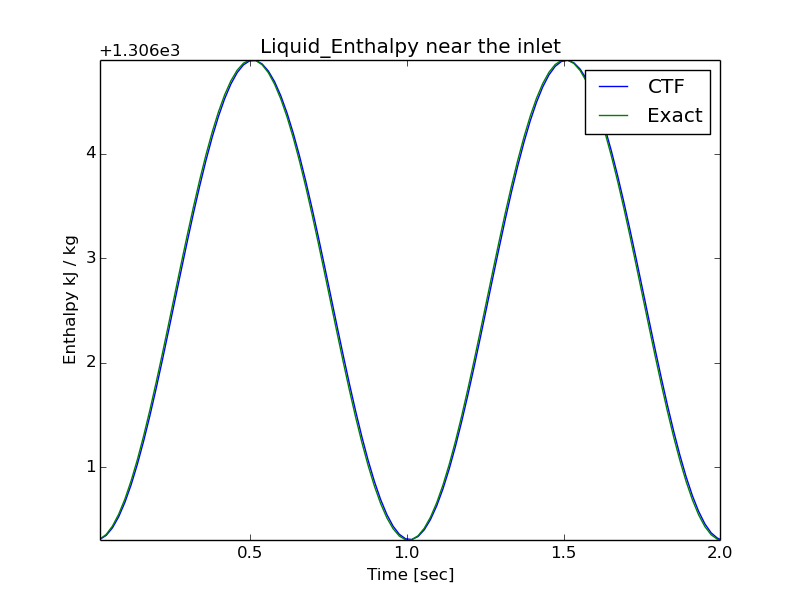
\includegraphics[width=0.675\textwidth]{images/Inlet_h}
	\caption{Enthalpy near the inlet and the analytical solution}
	\label{fig:Inlet_h}
\end{figure}

\begin{figure}[!h]
	\centering
	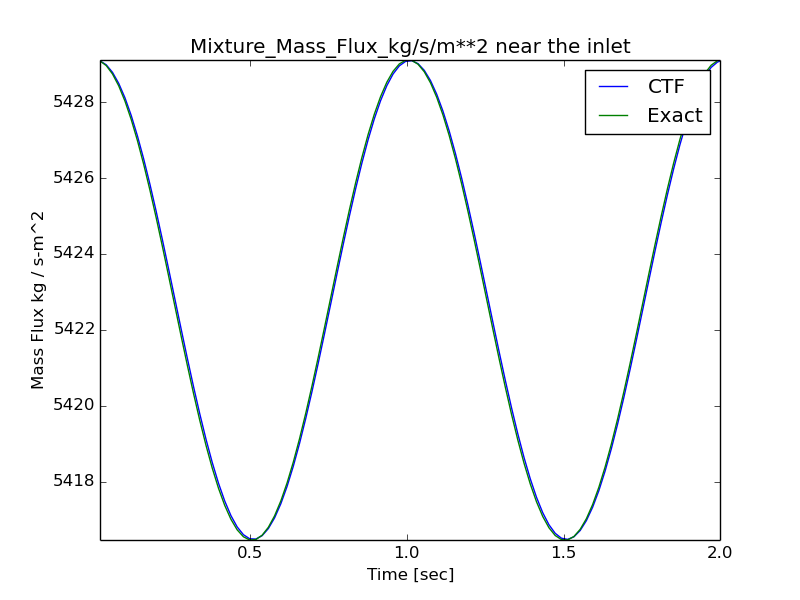
\includegraphics[width=0.675\textwidth]{images/Inlet_m_dot}
	\caption{Mass Flow rate near the inlet and the analytical solution}
	\label{fig:Inlet_m_dot}
\end{figure}

\section{Verification of All Solution Methods}

Both COBRA-TF and residual version semi-implicit method, residual fully implicit
method with and without linear EOS.

\subsection{Code Verification}

This compares the exact solution to the COBRA-TF Solution Methods

\subsubsection{Error Quantification}

Show qualatative plot and demonstrate that the error is quantified 
for a single time step and space discretization

A figure and a table of l1 normalized error

\subsection{Convergence of Error}

Show how error behaves for different time and space sizes

\subsection{Order of Accuracy}

%\section{Parameter Study}
%
%Tables and figures of varying the results.
%
%\subsection{Changes in $\Delta$T}
%
%This changes the amplitude of the displacement
%
%\subsection{Changes in Frequencey}
%
%This changes the frequencey of the displacement
%
%\subsection{Changes in Mass Flow Rate}
%
%\section{Computational Time}
%
%The computational time of the two methods for different computational sizes.
%Compare the semi-implicit and fully implicit methods at 0.5 , 1.0, and 2.0 CFL. 

\section{Conclusions}

Present your summary and conclusions here.

%%%%%%%%%%%%%%%%%%%%%%%%%%%%%%%%%%%%%%%%%%%%%%%%%%%%%%%%%%%%%%%%%%%%%
\section{Acknowledgments}

Dr. Vince Mosseau, Dr. Maria Avramova, Dr. Kostadin Ivanov, and Nathan Porter.

%%%%%%%%%%%%%%%%%%%%%%%%%%%%%%%%%%%%%%%%%%%%%%%%%%%%%%%%%%%%%%%%%%%%%
\setlength{\baselineskip}{12pt}

\bibliographystyle{mc2015}
\bibliography{references}

%%%%%%%%%%%%%%%%%%%%%%%%%%%%%%%%%%%%%%%%%%%%%%%%%%%%%%%%%%%%%%%%%%%%%

%\appendix
%\section{}


\end{document}
